\section{Integration into Rendering Software}
\label{sec:pn_rendering_integration}

This section will explain in detail how the solver and its result can be integrated and used in a standard rendering framework.

The solver framework is encapsulated using the \emph{PNSystemBuilder} class and therefore, can be easily migrated from a standalone application into any rendering framework. As outlined in section~\ref{sec:pn_framework}, references to a \emph{Stencil} class and the \emph{Scene} class are needed to create a \emph{PNSystemBuilder} instance.

The truncation order $N$ is a user parameter, which ideally is decided at runtime. However, the stencil code will always be the same for a given truncation order $N$, since it has been generated independently of grid resolution, boundary conditions and radiative transfer parameters. It suggests itself to precompute and precompile the stencil code for all possible options for $N$. The rendering framework is compiled once with all possible stencil codes. As soon as the user decided, which truncation order $N$ to use, a \emph{Stencil} class is generated using the function pointers of the respective compiled stencil code functions.

The \emph{Scene} class is also created by the rendering framework. It will be populated with references to \emph{Field} classes for radiative transfer quantities, such as extinction, albedo, emission and phase function. The \emph{Field} classes serve as adapter pattern according to Gamma et al.~\cite{Gamma95} and can be used to feed arbitrary representations of spatially varying scalar fields, as input to the solver framework.

An important aspect of providing inputs to the solver is the emission term, which describes the illumination within the problem domain. Light sources, which illuminate the volume from outside, will have to be expressed as emission on the boundary interface and light sources inside the problem domain, such as point- or area lights need to be rasterized into the emission field. Expressing outside illumination at the boundaries potentially conflicts with the boundary conditions, which cause the solution near the boundary to be less accurate. Rasterizing light sources inside the domain will be challenging for the solver, if strong directionality is present. The cause is the spherical harmonics approximation that has difficulties representing delta or strongly directional functions in angular domain due to truncation of higher frequency moments.

To alleviate the challenges of light sources with strong directionality, the rendering system, developed as part of this thesis, implements an idea, which is inspired by Grosjean’s analytical approximation to exact transport of a point light source within a homogeneous medium (Grosjean~\cite{Grosjean56}). Instead of providing an approximation to the full light transport caused by the point light, the approximation separates the unscattered light from the scattered light. The solution for the unscattered contribution is exact and an approximation is needed only for the scattered light. This approach is reasonable as the light contribution from scattered light has more energy in the lower frequencies due to the phase function, which acts as a convolution filter on the radiance function in angular domain.

Following this idea by Grosjean, the radiance field $L$ is separated into unscattered light $L_{u}$ and multiple scattered light $L_m$:
\begin{align}
L\left(\vec{x}, \omega\right) = 
L_u\left(\vec{x}, \omega\right)
+L_m\left(\vec{x}, \omega\right)
\end{align}

The unscattered light is the contribution of the radiance field, which did not undergo any scattering events. Therefore, it satisfies the following restricted radiative transfer equation, where the scattering term vanished:
\begin{align}
\left(\nabla\cdot\omega\right)L_u\left(\vec{x}, \omega \right)
=
-\sigma_t\left(\vec{x}\right) L_u\left(\vec{x}, \omega \right)
\label{eq:restricted_rte}
\end{align}


When replacing the radiance field $L$ with the decomposition above in the radiative transfer equation (equation~\ref{eq:rte}) the result is:
\begin{align}
\left(\nabla\cdot\omega\right)L_u\left(\vec{x}, \omega \right)
+\left(\nabla\cdot\omega\right)L_m\left(\vec{x}, \omega \right)
=&
-\sigma_t\left(\vec{x}\right) L_u\left(\vec{x}, \omega \right)
\nonumber\\
&
-\sigma_t\left(\vec{x}\right) L_m\left(\vec{x}, \omega \right)\nonumber\\
&
\underbrace
{
+\sigma_s\left(\vec{x}\right) \int_{\Omega}
{
\phase\left(\omega'\cdot\omega\right)L_u\left(\vec{x}, \omega' \right)\ud\omega'
}
}_{L_s}
\nonumber\\
&
+\sigma_s\left(\vec{x}\right) \int_{\Omega}
{
\phase\left(\omega'\cdot\omega\right)L_m\left(\vec{x}, \omega' \right)\ud\omega'
}
\nonumber
\\
&
+Q_e\left(\vec{x}, \omega\right)
\nonumber
\  .
\end{align}

By using equation~\ref{eq:restricted_rte}, the extinction terms for the unscattered light can be cancelled out, producing the medium radiative transfer equation:
\begin{align}
\left(\nabla\cdot\omega\right)L_m\left(\vec{x}, \omega \right)
=&
-\sigma_t\left(\vec{x}\right) L_m\left(\vec{x}, \omega \right)\nonumber\\
&
+\sigma_s\left(\vec{x}\right) \int_{\Omega}
{
\phase\left(\omega'\cdot\omega\right)L_m\left(\vec{x}, \omega' \right)\ud\omega'
}
\nonumber
\\
&
\underbrace
{
+L_s\left(\vec{x}, \omega\right)
+Q_e\left(\vec{x}, \omega\right)
}_{Q}
\nonumber
\  .
\end{align}
The quantity $L_s$ is the single scattered light, which is folded together with the volume emission $Q_e$ into the general emission term $Q$.

Using the emission term $Q$, the medium radiative transfer equation is solved, using the $P_N$-method previously described. The solution vector $\vec{u}$ is brought into collocated form, using the \emph{unstaggering} function described in section~\ref{sec:pn_staggered}. This allows straightforward subsequent use in a rendering system for image generation. 

The solution vector provided by the solver contains a set of spherical harmonics coefficients for every voxel of the computational grid. This set of coefficients describes the spherical radiance function at the voxelcenter. The framework, which has been developed as part of this thesis, provides a \emph{PNSolution} class that is a voxelgrid of $K$-dimensional vectors. The number of vector elements $K$ is the number of spherical harmonics coefficients, which is driven by the truncation order of the $P_N$-equations. The radiance field is reconstructed by first interpolating all coefficients at the given worldspace position from the coefficients at surrounding voxels, followed by computing the spherical harmonics reconstruction in equation~\ref{eq:sh_real_reconstruction}.

In this thesis, images will be rendered from the solution directly. An alternative route could be to use the solution in combination with one of the variance reduction techniques outlined in section~\ref{sec:foundations_mc}.

Volume rendering frameworks are concerned with solving the radiative transfer equation~\ref{eq:rte}. In order to integrate the solution of the medium radiative transfer equation, the inscattering term in the radiative transfer equation has to be split and the medium radiance $L_m$ is replaced by its truncated spherical harmonics reconstruction $\widehat{L}_m$:
\begin{align}
\left(\nabla\cdot\omega\right)L\left(\vec{x}, \omega \right)
=&
-\sigma_t\left(\vec{x}\right) L\left(\vec{x}, \omega \right)\nonumber\\
&
+\sigma_s\left(\vec{x}\right) \int_{\Omega}
{
\phase\left(\omega'\cdot\omega\right)\left(L_u\left(\vec{x}, \omega' \right)+\widehat{L}_m\left(\vec{x}, \omega' \right)\right)\ud\omega'
}
\nonumber
\\
&
+Q_e\left(\vec{x}, \omega\right)
\nonumber
\\
=&
-\sigma_t\left(\vec{x}\right) L\left(\vec{x}, \omega \right)
\nonumber\\
&
+\sigma_s\left(\vec{x}\right) \int_{\Omega}
{
\phase\left(\omega'\cdot\omega\right)L_u\left(\vec{x}, \omega' \right)\ud\omega'
}
\nonumber\\
&
+\sigma_s\left(\vec{x}\right) \int_{\Omega}
{
\phase\left(\omega'\cdot\omega\right)\widehat{L}_m\left(\vec{x}, \omega' \right)\ud\omega'
}
\nonumber\\
&
+Q_e\left(\vec{x}, \omega\right)
\label{eq:pn_rendering_integration1}
\end{align}
When seperating the radiance field and using the single scattered light as emission term for the $P_N$-method, this equation needs to be solved to fully account for the radiance field. Any Monte-Carlo method would need to integrate the single scattered light (e.g. by doing next event estimation). The indirect or multiple scattered light is accounted for by integrating over the angular dependent $P_N$-solution and weighting it by the phase function and scattering term to account for the inscattering of indirect illumination.

If the phase function is isotropic, then equation~\ref{eq:pn_rendering_integration1} further simplifies to
\begin{align}
\left(\nabla\cdot\omega\right)L\left(\vec{x}, \omega \right)
=&
-\sigma_t\left(\vec{x}\right) L\left(\vec{x}, \omega \right)
+\sigma_s\left(\vec{x}\right) \int_{\Omega}
{
\phase\left(\omega'\cdot\omega\right)L_u\left(\vec{x}, \omega' \right)\ud\omega'
}
\nonumber\\
&
+
\frac{1}{4\pi}
\sigma_s\left(\vec{x}\right)
\int_{\Omega}
{
\widehat{L}_m\left(\vec{x}, \omega' \right)\ud\omega'
}
+Q_e\left(\vec{x}, \omega\right)
\nonumber\\
=&
-\sigma_t\left(\vec{x}\right) L\left(\vec{x}, \omega \right)
+\sigma_s\left(\vec{x}\right) \int_{\Omega}
{
\phase\left(\omega'\cdot\omega\right)L_u\left(\vec{x}, \omega' \right)\ud\omega'
}
\nonumber\\
&
+
\frac{1}{4\pi}
\sigma_s\left(\vec{x}\right)
L_m^{0,0}\left(\vec{x}\right)
+Q_e\left(\vec{x}, \omega\right)
\ ,
\label{eq:pn_rendering_integration2}
\end{align}
due to zero moment property of the radiance field $\int_{\Omega}\widehat{L}_m\ud\omega'=L_m^{0,0}$.

Figure~\ref{fig:pn_rendering_integration_overview} gives a schematic overview over how the method is integrated into a rendering framework. The single scattered light is precomputed and projected into the emission term for the $P_N$-solver. Together with the other discretized radiative transfer parameters, the $P_N$-solution is obtained. The final image is generated by path tracing to the first bounce into the volume, and by computing the inscattered uncollided light (either by using Monte Carlo integration or by using the precomputed single scattered light, which was used as emission term for the $P_N$-solver). Instead of continuing tracing the path to account for indirect illumination, a separate inscattering integral is computed over the multiple scattered light from the $P_N$-solution.

\begin{figure}[h]
\centering
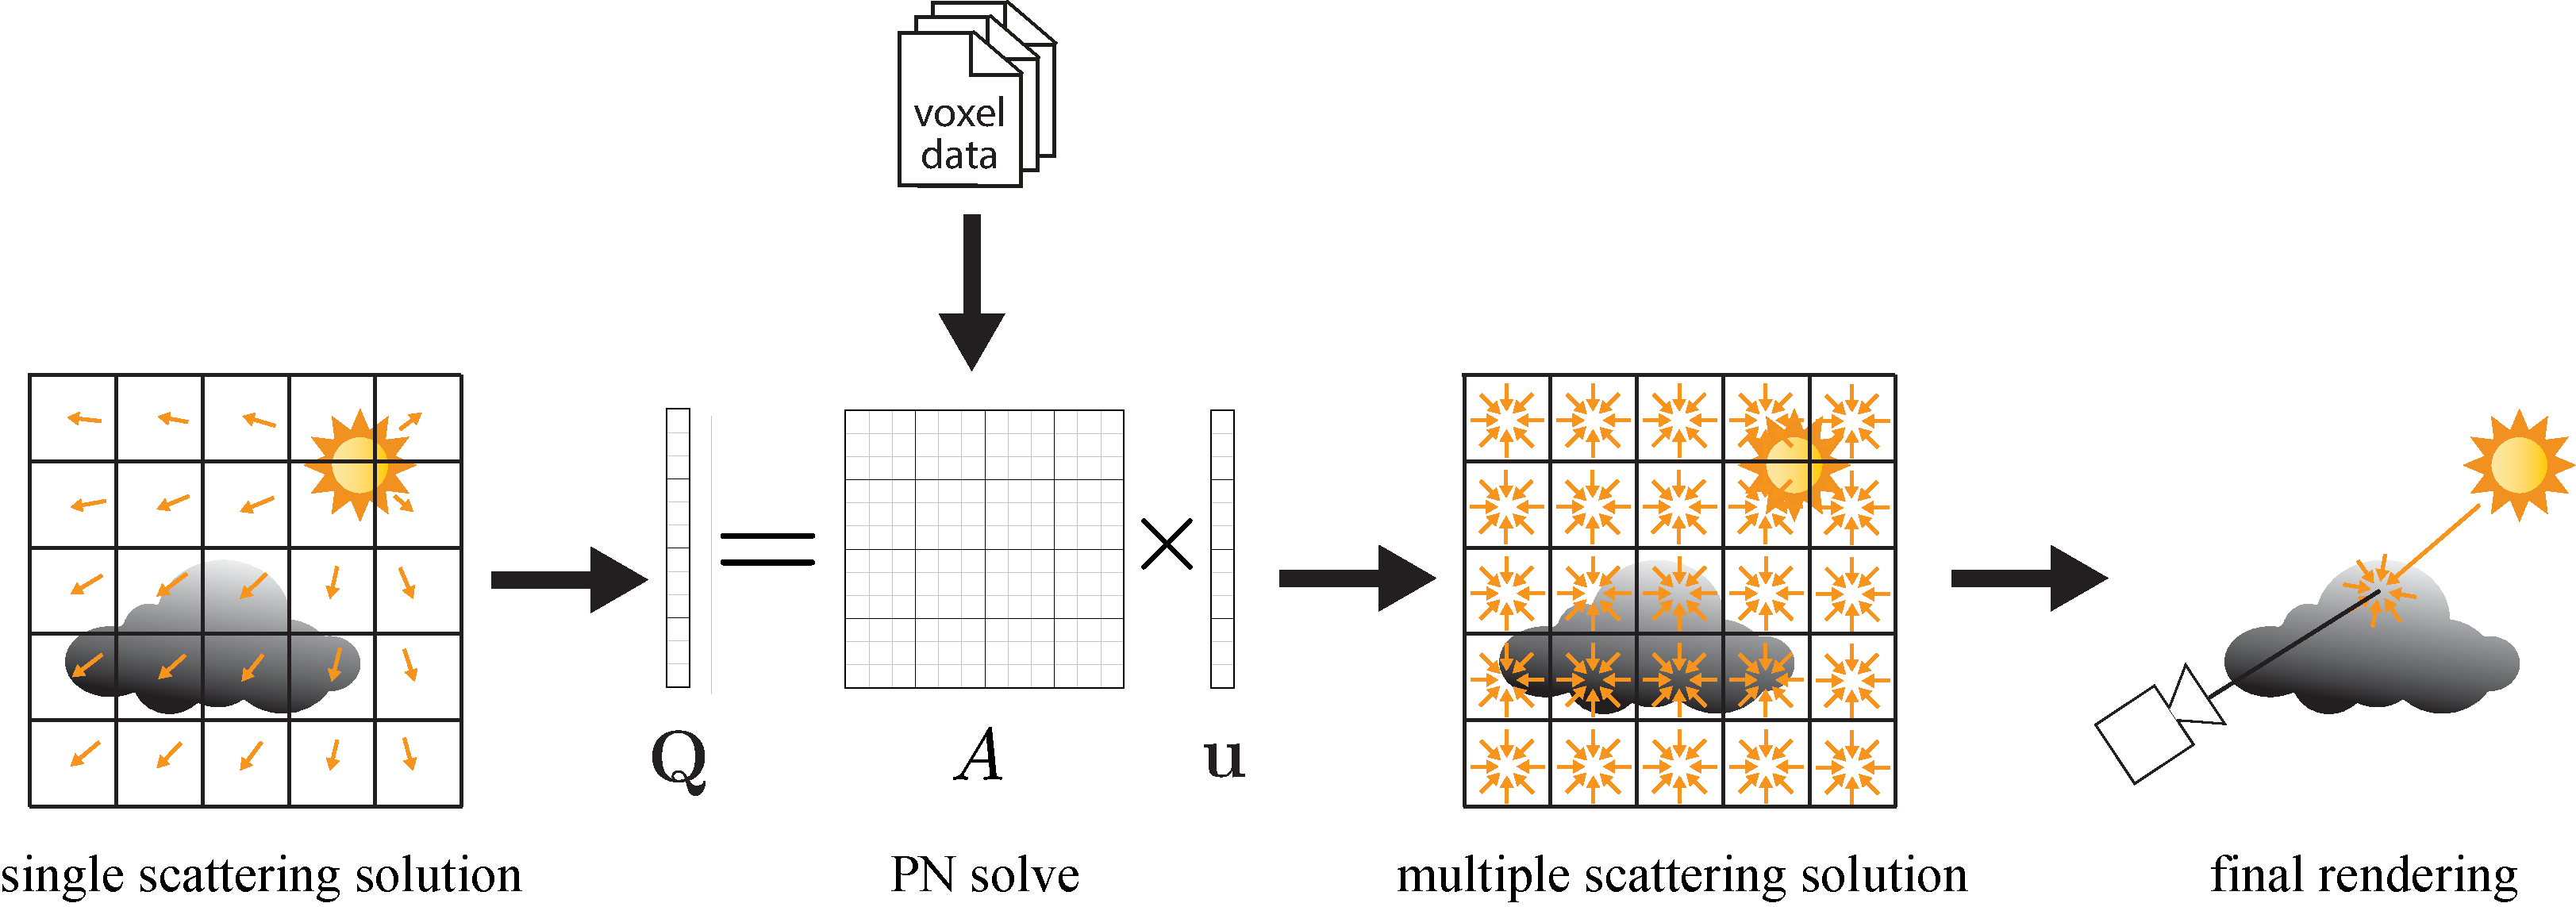
\includegraphics[width=0.99\textwidth]{04_pn_method/figures/fig_rendering_pipeline.pdf}
%\missingfigure{show high level picture of a rendering system. input data. precomputation. rasterization. synthesis of first order scattering and higher order scattering}
\caption{Overview over the full rendering process. The single scattering solution is precomputed and projected into RHS $Q$. The coefficient matrix $A$ is assembled from voxelized RTE quantities and used to compute solution $u$. That solution is then un-projected and used to evaluate the multiple scattering contribution during final rendering step.}
\label{fig:pn_rendering_integration_overview}
\end{figure}

After having outlined how the $P_N$-Method and its solution can be integrated into a rendering application, concrete results will be shown and discussed in the following section.
